\subsection{Keypoint-Based Visual SLAM}
\label{sec:kv_slam_background}

SLAM is the joint problem of simultaneously generating a map of an environment and estimating the position of an observer within that map based on sensor observations. First explored in the 1980s \cite{smithEstimatingUncertainSpatial1988}, SLAM has become a de facto standard in robotics for tasks which require operations within unfamiliar environments. A wide variety of sensors can be utilized by SLAM, the most common being LiDAR, cameras, and RGBD sensors. The high level relationships between these sensor modalities are shown in Figure \ref{fig:slam_family_tree}. Keypoint-Based Visual SLAM refers to a subset of the wider SLAM ecosystem characterized by the use of cameras as the primary sensor, and image features extracted from images as the primary data for tracking and mapping.

\begin{figure}[!ht]
    \centering
    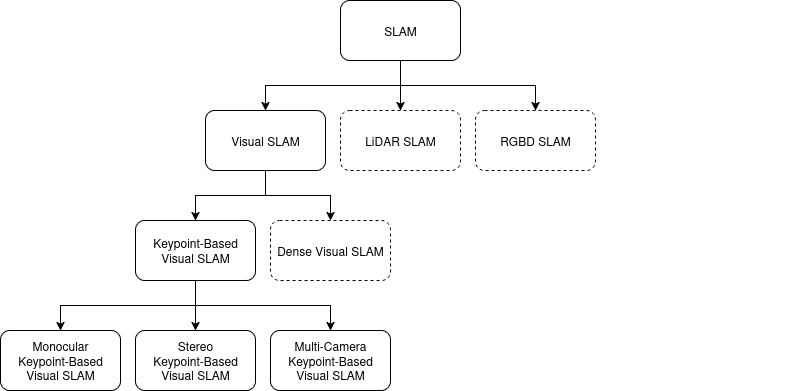
\includegraphics[width=0.8\textwidth]{resources/slam_family_tree.png}
    \caption[SLAM Family Tree]{Overview of the relationships between popular SLAM modalities.}
    \label{fig:slam_family_tree}
\end{figure}

The first implementations of KV-SLAM came in the early 2000s \cite{seMobileRobotLocalization2002}\cite{davisonRealtimeSimultaneousLocalisation2003}, making the field relatively young. This can be attributed to the difficulty in estimating 3D geometries from 2D images, unlike LiDAR and RGBD which are capable of direct 3D environmental measurements. However, due to the extremely low cost and wide availability of camera sensors, KV-SLAM is a popular modality for robotics, AR/VR, and autonomous driving applications. A full description of the internal operations of KV-SLAM is out of scope for this thesis, but an overview of key concepts relevant to this research is given below, followed by an overview of the relevant portions of the SLAM pipeline.

\subsubsection{Image Features}

An image feature is the combination of a keypoint and a feature descriptor \cite{loweObjectRecognitionLocal1999}. Keypoints are locations in an image which are (ideally) invariant to lighting, scale, translation, and rotation\cite{shiGoodFeaturesTrack1994}, while descriptors are a data vector that acts as the unique fingerprint for the feature. Keypoints are located, and their descriptors generated in a process called feature extraction.

The output of feature extraction is a set of image features, which when combined are significantly smaller than the image from which they were extracted. Figure \ref{fig:feature_extraction_and_matching} shows the output of the ORB feature extractor, along with how the features extracted between two images can be matched by their descriptors.

\begin{figure}[!ht]
    \centering
    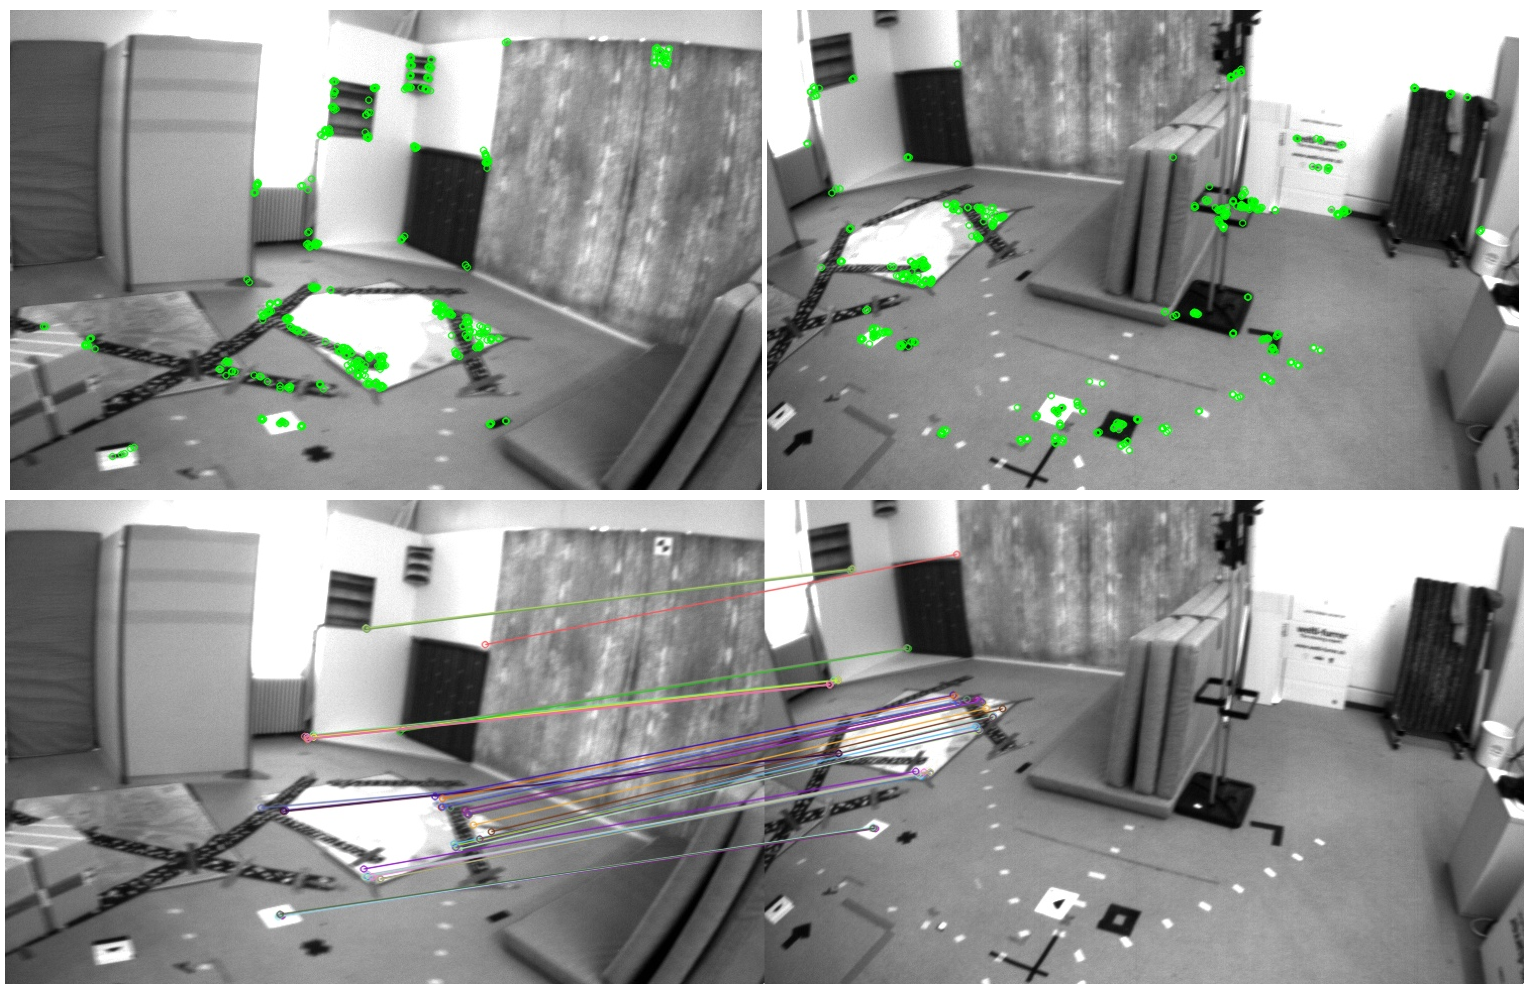
\includegraphics[width=0.8\textwidth]{resources/feature_extraction_and_matching.png}
    \caption[Image Feature Extraction and Matching]{(Top) ORB features extracted from two frames of the EuRoC MAV V1\_03 dataset.}
    \label{fig:feature_extraction_and_matching}
\end{figure}

\subsubsection{RANSAC}

% What is SLAM? What are its goals? What are its use cases?
SLAM refers to the joint problem of simultaneously generating a map of an environment and estimating the position of an observer within that map based on sensor observations. With research beginning in the 1980s \cite{smithEstimatingUncertainSpatial1988}, SLAM has become a de facto standard in robotics for tasks which require operations within unfamiliar environments. The benefit of SLAM when compared to other navigation methods such as pure localization is the ability to operate with no a-prioiri information, instead creating and incrementally updating the map at runtime. The selection of sensors is extremely flexible, with many popular implementations existing for camera, LIDAR, and RGBD based sensor modalities. Through careful selection of sensors, SLAM systems can operate in a wide variety of environments, from indoor office spaces to densely forested areas, and even underwater or in space.  These features make SLAM a powerful too for autonomous navigation, leading to its widespread use in robotics, augmented reality, and autonomous vehicles.

% What are the defining characteristics of keypoint based visual SLAM as opposed to other SLAM methods?
This research targets Keypoint-Based Visual SLAM (KV-SLAM), a specific modality of SLAM characterized by its use of one or more cameras as the primary sensor, and the use of keypoints as opposed to raw pixel values as the primary data for constructing the map and performing localization. As opposed to other sensor modalities such as LIDAR and RGBD, which take direct 3D measurements of the environment, KV-SLAM relies on the principles of epipolar geometry to infer depth and camera motion from the relative position of keypoints between image frames. The map generated by a KV-SLAM system is a sparse point cloud of 3D map points. Core to this research is the concept of the keypoint, map point, and sparse map, motivating a discussion on the definitions and structure of these types, and how they relate to the larger KV-SLAM pipeline.


% Describe the structure of a map in kvSKAM, including keyframes, map points, and their relationships.
The primary input to a KV-SLAM system is the keypoint. A keypoint is the combination of an image feature and a descriptor. Image features can take many forms, but for the purposes of SLAM, they should be identifiable, meaning they are quick to compute, and differentiable, meaning they are unique enough to tell one instance of a feature from another. Image features are differentiated using a descriptor, which is a vector representation of the feature that captures its unique characteristics. Ideally, keypoints should be invariant to changes in scale, rotation, and illumination, allowing them to be reliably matched between images taken from different viewpoints or under different lighting conditions.

Map points represent the extrapolation of keypoints into 3D space. Two views of the same set of keypoints can be used to triangulate the 3D position of the visual feature, in conjunction with the camera transformation between the two views. Depending on the implementation, map points often store additional metadata, such as the set frames in which they were observed, the descriptors of the keypoints they were derived from, etc. The primary contribution of this research is a novel method of determining and representing the observability of map points at the individual point level, allowing for the efficient and accurate identification of outdated map points.

The sparse map is the collection of all map points, acting as a 3D representation of the environment. It is used to localize new frames by finding a transformation that aligns the currently seen keypoints with the existing map points. This 2D-3D alignment is accomplished through an optimization process which iteratively refines the camera transform to minimize the reprojection error between the matched features.

% Explain how data flows through a keypoint-based visual SLAM system, from sensor input to map and pose output.
With these structures in hand, we can describe the pipeline which data follows through a generic KV-SLAM system. A graphical representation of the pipeline can be seen in Figure \ref{fig:kv_slam_pipeline}, each stage is expanded on here.

1. Initialization

\begin{figure}[!ht]
    \centering
    % \includegraphics[width=0.8\textwidth]{figures/kv_slam_pipeline}
    \caption{Keypoint-based Visual SLAM pipeline showing the flow of data from sensor input to map and pose output.}
    \label{fig:kv_slam_pipeline}
\end{figure}

% High level overview of the challenges of SLAM: computational complexity, sensor error accumulation, dynamic environments
This high-level overview of KV-SLAM Despite numerous advancements, the computational complexity of performing SLAM in real-time remains a challenge, meaning that on many resource constrained platforms, implementations can struggle to keep up with the rate of sensor data acquisition \cite{semenovaQuantitativeAnalysisSystem2022}. Additionally, because there is no fixed reference, SLAM systems can suffer from sensor error accumulation, leading to inaccurate maps and poses over time \cite{cadenaPresentFutureSimultaneous2016}. These issues are compounded as the timeframe, scale, and environmental dynamics of the SLAM task increase. Larger environments require larger, more complex maps, which produce higher computational load and longer processing times. Dynamic environments, where objects can move or change either during the SLAM process or between runs, are a particular challenge, as most SLAM systems tend to operate best in static environments, and can struggle to maintain accurate pose estimation and map consistence in the presence of moving objects. The field of SLAM research known as \textit{lifelong SLAM} \cite{cadenaPresentFutureSimultaneous2016} focuses on addressing these challenges, and will be covered in detail in Section \ref{sec:related_work}.
